% !TEX root = ../thesis.tex

\chapter{Introduction \& Motivation} \label{chp:intro}

Quantum computers represent information as quantum states, and for specific problems they may asymptotically outperform known classical algorithms~\cite{NielsenChuang2010}.
Quantum computation was first suggested as an efficient method to simulate quantum systems ~\cite{feynman1982,lloyd1996}.
The premise is simple: to exactly represent $N$ two-state quantum systems requires memory scaling of $\mathcal{O}(2^N)$, but it would require only $N$ physical two state quantum systems.
Simulating quantum systems remains one of the most promising applications, with problems of interest across chemistry and materials science~\cite{bauer2020}.
% Proposed applications also extend to optimization, finance, and machine learning~\cite{montanaro2016, dalzell2025}.
That being said, the most famous application of a quantum computer is Shor's algorithm, which offers an exponential speedup for factoring numbers and would break widely used public-key cryptography~\cite{shorAlgorithmsQuantumComputation1994}.
% Grover's algorithm also gives a quadratic speedup for unstructured search problems~\cite{groverFastQuantumMechanical1996}.

Realizing these algorithms at a useful scale requires a large-scale, fault-tolerant quantum computer, and such active error correction comes with substantial overhead.
The threshold theorem guarantees that logical errors can be suppressed arbitrarily, provided the physical error rate $p$ lies below a threshold $p_{\rm th}$~\cite{aharonov2008,knill1998}.
How far below matters.
In the surface code, for example, the logical error rate falls as $(p/p_{\rm th})^{(d+1)/2}$ with code distance $d$, so better physical qubits reach a target logical error rate with a smaller code and far fewer physical qubits per logical qubit~\cite{fowler2012}.
Reducing this overhead, through better physical qubits and more efficient codes, is central to the field.

\section{Superconducting Qubits}

% Platform in one paragraph; cite full treatments for the basics rather than re-deriving them~\cite{blaisCircuitQuantumElectrodynamics2021a,krantzQuantumEngineersGuide2019a,rasmussenSuperconductingCircuitCompanionan2021a}.

One of the most promising technologies to realize a fault tolerant quantum computer is superconducting Josephson junction circuits.
Cooled to millikelvin temperatures, these circuits behave as quantum systems, and two of their energy levels can be isolated and used as a qubit~\cite{clarke2008,devoret2013}.
They are often called artificial atoms, because their spectrum is set by the circuit design rather than fixed by nature.
Superconducting circuits also host bosonic encodings in the modes of microwave cavities~\cite{joshi2021}, which are not the focus of this thesis.

We now quickly review the development of these systems and establish where they stand today.
The first superconducting qubits were the Cooper pair box~\cite{bouchiat1998,nakamura1999} and the persistent-current flux qubit~\cite{mooij1999,vanderwal2000}, which were highly sensitive to charge and flux noise, respectively.
Indeed, the first coherent oscillations of a Cooper pair box were observed for only about $2$~ns~\cite{nakamura1999}.
Two designs that reduce these sensitivities underlie most qubits in use today (\cref{fig:single_mode_circuits}).
The transmon shunts the junction with a large capacitance, which suppresses its sensitivity to charge noise exponentially at the cost of a small anharmonicity~\cite{kochChargeinsensitiveQubitDesign2007b}.
The fluxonium instead shunts the junction with a large inductance~\cite{manucharyanFluxoniumSingleCooperPair2009a}, which gives a large anharmonicity and low qubit frequency, at the cost of flux noise sensitivity.
Both now reach millisecond coherence, with $T_2^* = 1.48$~ms in a fluxonium~\cite{somoroff2023} and $T_1$ up to $1.68$~ms in transmons~\cite{bland2025}.
For a more thorough introduction to circuit quantum electrodynamics (\cqed), including gates, readout, and experimental considerations, many excellent reviews and tutorials have been published~\cite{blaisCircuitQuantumElectrodynamics2021a,krantzQuantumEngineersGuide2019a,rasmussenSuperconductingCircuitCompanionan2021a,voolIntroductionQuantumElectromagnetic2017, Wang2021}.


The last few years have additionally seen substantial improvements in scaling and quantum error correction of superconducting systems.
Bosonic encodings had already reached memory break-even with a cat code in 2016~\cite{ofek2016}.
Subsequent experiments demonstrated logical lifetimes exceeding those of the best available physical encodings by factors of $2.27$ and approximately $1.16$ using Gottesman--Kitaev--Preskill (GKP) and binomial codes, respectively~\cite{sivak2023,ni2023}.
Progress with arrays of superconducting qubits has followed a similar route.
Repeated extraction of both bit- and phase-error syndromes was first demonstrated in a distance-three surface code in 2022~\cite{krinner2022}. In 2025, a beyond threshold surface code demonstration showed decreasing error rates with increasing surface code distance \cite{google2025}.


Despite these recent successes, it may pay off to investigate superconducting qubit systems with lower physical gate error rates~\cite{eisert2025}.
There are two complementary paths towards fault tolerance: lower-error physical qubits and better codes.
The lower the physical error rate or the better the code, the fewer physical qubits are needed.
This thesis concerns analyzing and identifying lower-error superconducting qubits.

% These advances have also broadened the architectures available for quantum error correction.
% Concatenating superconducting cat qubits with a repetition code combines intrinsic bit-flip suppression with active correction of phase errors, providing a route to reducing the hardware overhead of logical qubits~\cite{putterman2025}.
% Related progress includes logical entangled-state preparation outperforming its physical counterpart in trapped ions~\cite{hong2024}, below-threshold surface-code performance in neutral-atom arrays~\cite{bluvstein2026}, and repetition-code error suppression together with postselected quantum error detection in silicon spin qubits~\cite{hrl2026}.
% Selected results are summarized in \cref{tab:selected_qec}, distinguishing memory-lifetime gains from state-preparation advantages and code-distance scaling.
% Together, these experiments establish the practical benefit of encoding and correcting quantum information while motivating further improvements in physical-qubit design, control, and integration to reduce the resources required for large-scale fault-tolerant computation.

% Close: codes are the main route, but their overhead is set by the physical qubits underneath.


\section{Protected Qubits}\label{sec:protected_qubits}

Protected qubits suppress errors at the hardware level and represent a promising path towards lower error qubits \cite{gyenisMovingTransmonNoiseProtected2021b}.
The key is that the qubit states are insensitive to the local operators through which noise couples to the circuit.
We now examine this criteria in more detail.

\subsection{Decay and Dephasing}
\label{sec:estimating_lifetimes}

Energy-relaxation (and excitation) arise when a quantum system couples to a noisy environmental bath.
To first order, the system-bath interaction has the form $H_{\rm int} =\lambda(t)\hat O_\lambda$, where $\lambda (t)$ represents a noisy parameter, and
\begin{equation}
	\hat O_\lambda
	=
	\frac{\partial \hat H}{\partial\lambda}
\end{equation}
is the operator to which the noise couples.
Fermi's golden rule gives the downward transition rate between two eigenstates $\ket{i}$ and $\ket{j}$ of the Hamiltonian $\hat H$:
\begin{equation}
	\Gamma_{j \rightarrow i}^{(\lambda)}
	=
	\frac{1}{\hbar^2}
	\left|
		\bra{i} \hat O_\lambda \ket{j}
	\right|^2
	S_\lambda(\omega_{ij}),
	\label{eq:fermi-golden-rule-relaxation}
\end{equation}
where $S_\lambda(\omega)=\int_{-\infty}^{\infty}dt\,e^{-i\omega t}\langle\lambda(0)\lambda(t)\rangle$ is the noise spectral density and $\omega_{ij}=(E_j-E_i)/\hbar$ is the transition frequency~\cite{groszkowski2018}.
The logical states are protected against energy relaxation if, for every logical state $\ket{j}$ and every state $\ket{i}$ below it, logical or not,
\begin{align}
    \bra{i} \hat O_\lambda \ket{j} = \mathcal O\big(e^{-\xi}\big)
\end{align}
is exponentially suppressed in a system design parameter $\xi$ that can be made large.
Decay into a non-logical state is leakage, so it must be suppressed as well as decay between logical states.
In the soft \zps qubit, for example, the logical states are $\ket{0}$ and $\ket{2}$, so $\ket{2}$ must decay slowly into both $\ket{0}$ and $\ket{1}$  (see \cref{chp:zp_2q_gates}).
Such suppression typically follows from nearly disjoint support of the logical wavefunctions, because the common noise operators, such as $\hat n$ and $\hat\phi$, act locally~\cite{gyenisMovingTransmonNoiseProtected2021b}.

Dephasing arises from slow fluctuations of a noisy parameter, which leads to shifting energy eigenvalues.
First-order sensitivity of the $\ket{i} \leftrightarrow \ket{j}$ transition to dephasing is set by the derivative of the transition frequency with respect to the noisy parameter~\cite{ithier2005}
\begin{equation}
	D_{ij}^{(\lambda)}
	\equiv
	\frac{\partial \omega_{ij}}{\partial\lambda}
	=
	\frac{1}{\hbar}
	\left(
	\bra{j} \hat O_\lambda \ket{j}
 	-
	\bra{i} \hat O_\lambda \ket{i}
	\right)
	\, .
\label{eq:dephasing-sensitivity}
\end{equation}
The second equality follows from the Feynman--Hellmann theorem. If ${\partial \omega_{ij}}/{\partial\lambda} = 0$, the qubit is at a sweet spot and the leading sensitivity is determined by $\partial_\lambda^2\omega_{01}$. The dephasing rate is proportional to the sensitivity squared $\Gamma^{(\lambda)}_{\varphi, ij } \propto |D_{ij}^{(\lambda)}|^2$.
A qudit is protected against dephasing if for all combinations of logical states $\ket{i}, \ket{j}$,
\begin{align}
    \frac{\partial \omega_{ij}}{\partial\lambda} = \mathcal O\!\left(e^{-\eta}\right)
\end{align}
is exponentially suppressed in a system design parameter $\eta$ that can also be made large.
Equivalently, the total dispersion of $\omega_{ij}$ over the range of $\lambda$ is exponentially small.
Following \textcite{gyenisMovingTransmonNoiseProtected2021b}, we call protection exponential when these conditions hold, and sweet-spot protection when only the first derivative of $\omega_{ij}$ vanishes at the operating point.

Relaxation and dephasing together set the total coherence time $T_2 = 1/(2\Gamma_\varphi +\Gamma_1)= \left[1/(2T_1) + 1/T_\varphi\right]^{-1}$, for $T_1=1/\Gamma$ and $T_\varphi=1/2\Gamma_\varphi$.




\subsection{Single-Mode Qubits}
\label{sec:single_mode_protection}

\begin{figure}[ht!]
    \centering
    % Panel letters sit inside each panel (top left); the subfloat captions are hidden but still number the panels.
    \captionsetup[subfloat]{labelformat=empty, captionskip=0pt, nearskip=0pt, farskip=4pt}
    \newcommand{\panel}[2]{\begin{tikzpicture}
        \node[inner sep=0pt] (p) {#2};
        \node[anchor=north west, inner sep=0pt, font=\small] at (p.north west) {(#1)};
    \end{tikzpicture}}
    % Two aligned rows, (a) (c) over (b) (d); the counter is set so the panels still number a--d.
    % The heatmaps share one scale; (b) has no E_L = 0 strip, so it is narrower.
    \newlength{\panelw}\setlength{\panelw}{0.49\textwidth}
    \setcounter{subfigure}{0}%
    \subfloat[\label{fig:single_mode_circuits}]{\panel{a}{\includestandalone[width=\panelw]{chapter-1-intro-background/figs/single_mode_qubits}}}\hfill
    \setcounter{subfigure}{2}%
    \subfloat[\label{fig:single_mode_n01}]{\panel{c}{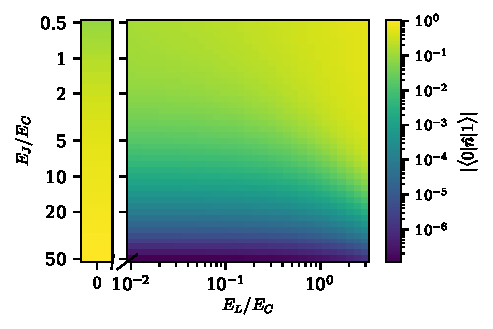
\includegraphics[width=\panelw]{chapter-1-intro-background/figs/single_mode_n01.pdf}}}\\
    \setcounter{subfigure}{1}%
    \subfloat[\label{fig:single_mode_phi01}]{\makebox[\panelw][r]{\panel{b}{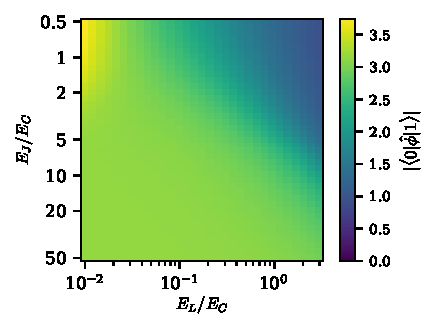
\includegraphics[width=0.8827\panelw]{chapter-1-intro-background/figs/single_mode_phi01.pdf}}}}\hfill
    \setcounter{subfigure}{3}%
    \subfloat[\label{fig:single_mode_curvature}]{\panel{d}{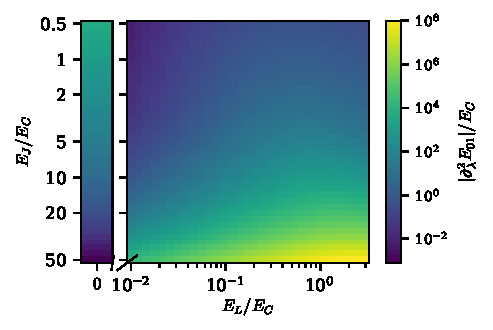
\includegraphics[width=\panelw]{chapter-1-intro-background/figs/single_mode_curvature.pdf}}}
    \caption[Single-mode superconducting qubits and their protection]{(a) Single-mode superconducting qubits, arranged by $E_J/E_C$ and $E_L/E_C$ as in (b)--(d).
    Adding capacitance moves a circuit down, and adding an inductance moves it to the left (an infinitely large inductor is an open circuit).
    (b), (c) Transition matrix elements, which set the coupling to flux and charge noise that causes decay.
    (d) Sweet-spot curvature, which sets the second-order sensitivity of the qubit frequency to that noise.
    Strips at $E_L = 0$ are the Cooper pair box and transmon at $n_g = 0$ ($\lambda = n_g$), and maps are the fluxonium at $\phi_{\rm ext} = \pi$, with energies in units of $E_C$.}
    \label{fig:single_mode_qubits}
\end{figure}

% \begin{table}[ht!]
%     \centering
%     \small
%     \begin{tabular}{>{\raggedright\arraybackslash}p{2.8cm}>{\raggedright\arraybackslash}p{4.6cm}ccc}
%         \toprule
%         Circuit & Logical states & $T_1$ & $T_\varphi$ ($n_g$) & $T_\varphi$ ($\Phi_{\rm ext}$) \\
%         \midrule
%         Cooper pair box & localized in charge & absent & sweet spot & --- \\
%         Transmon & localized in phase & absent & exponential & --- \\
%         Fluxonium & delocalized across neighboring wells & absent & exponential* & sweet spot \\
%         Heavy fluxonium & localized in single wells, away from $\Phi_0/2$ & exponential & exponential* & absent \\
%         \bottomrule
%     \end{tabular}
%     \caption[Protection of single-mode qubits]{Protection of the single-mode qubits of \cref{fig:single_mode_circuits}.
%     The transmon, fluxonium and heavy fluxonium entries are from Table~I of \textcite{gyenisMovingTransmonNoiseProtected2021b}.
%     Absent: no protection; sweet spot: first-order insensitivity; exponential: exponential suppression; ---: the circuit does not couple to this parameter.
%     Exponential*: exponential insensitivity to offset charge from coherent quantum phase slips in the junction-array superinductance~\cite{gyenisMovingTransmonNoiseProtected2021b}.}
%     \label{tab:single_mode_protection}
% \end{table}

The single-mode qubits of \cref{fig:single_mode_circuits} are each built from one junction, a capacitor, and at most one inductor.
\Cref{fig:single_mode_n01,fig:single_mode_phi01} show the transition matrix elements that set relaxation, and \cref{fig:single_mode_curvature} shows the sweet-spot curvature that sets dephasing.
None of these circuits are protected against both relaxation and dephasing.
Any region in parameter space where one quantity is suppressed is unsuppressed in another.

The key is that a single mode offers only one coordinate in which to arrange the two logical wavefunctions.
Exponentially small matrix elements require disjoint support, which corresponds to localized (and non-overlapping) logical states in the relevant coordinate.
Exponentially small dispersion instead requires the logical states to be delocalized so that a small shift in the coordinate has little effect.
Such states typically have large overlap, so they are connected strongly by local matrix elements.
Protection against both requires either a second mode, so that the logical states can be disjoint in one coordinate and delocalized in another \cite{gyenisMovingTransmonNoiseProtected2021b}, or additional circuit elements, which we examine next.

\subsection{The \texorpdfstring{$\cos 2\phi$}{cos 2φ} Qubit}
\label{sec:cos2phi}

The argument above assumes that the circuit is built from Josephson junctions, capacitors, and inductors.
A single mode can be protected against both relaxation and dephasing if its junction is replaced by an element that tunnels only pairs of Cooper pairs~\cite{gyenisMovingTransmonNoiseProtected2021b,smithSuperconductingCircuitProtected2020b}:
\begin{equation}
	\hat H
	=
	4 E_C \left(\hat n - n_g\right)^2
	-
	E_J \cos 2\hat\phi
	.
	\label{eq:cos2phi}
\end{equation}
The $\cos 2\hat\phi$ term changes $\hat n$ by $\pm 2$, so $\hat H$ conserves the charge parity $(-1)^{\hat n}$.
Its two lowest eigenstates are supported on even and odd charge states, respectively, so any noise operator that is a function of $\hat n$ has an exactly zero matrix element.
This is disjoint support enforced by symmetry.
In the phase basis, the potential has minima at $\phi = 0$ and $\pi$, and for $E_J \gg E_C$ the two eigenstates are the even and odd superpositions of states localized in these wells.
Tunneling splits the pair by $E_1 - E_0 \approx 4t|\cos(\pi n_g)|$, where $t \propto e^{-\sqrt{2E_J/E_C}}$ is the tunneling amplitude along each of the two paths between the wells.

No single element tunnels only pairs of Cooper pairs, so $\cos 2\phi$ qubits are approximated by multi-mode circuits whose low-energy dynamics approximate \cref{eq:cos2phi}.
For example, the \zps qubit has an effective $\cos 2\phase$ potential in one mode \cite{brooks2013,Dempster2014understanding,groszkowski2018,paolo_control_2019}. Only a ``soft'' version has been realized experimentally \cite{Gyenis_zero_pi_2021a}, which remains sensitive to dephasing.
Other circuits, like the Josephson rhombus \cite{Bell2014} and the KITE \cite{smithSuperconductingCircuitProtected2020b}, cancel single Cooper pair tunneling by interference at a particular flux bias.
Both have seen recent experimental implementations \cite{sanchezRevisitingMultimodeRhombus2026a, Roverch2026experimental}, but the demonstrations fall short of simultaneous protection against both decay and dephasing. 
We examine approximate $\cos 2\phase$ implementations in more detail in \cref{chp:rotor_codes}, where we show that circuit symmetries lead to a selection rule for first order flux noise protection, which limits the performance of both of the aforementioned experiments.


\FloatBarrier

\section{This Thesis}\label{sec:thesis_outline}

Protection requires multimode circuits, and multimode circuits are difficult to quantize, simulate, search over, and control.
This thesis addresses each of these in turn.
\Cref{chp:circuit_quantization} gives a general procedure to go from a circuit diagram to a multimode Hamiltonian, which every later chapter starts from.
This is not as straightforward as writing down the energy stored in each element.
The procedure must separate modes with periodic coordinates from those with real-valued coordinates, identify non-dynamical modes, and handle time dependent external flux.
The final choice of coordinates represents a residual freedom that decides how the Hamiltonian presents symbolically and how quickly it can be diagonalized numerically.
The chapter also summarizes this numerical treatment.
\Cref{chp:enumeration} searches over circuits, by enumerating all unique circuits built from a given set of elements and sorting them by the structure of their Hamiltonian, using a consistent choice of the final coordinates.
Earlier work on circuit equivalence compares circuits at a port, through an impedance or a transfer function.
Here two circuits are equivalent when they have the same quantized Hamiltonian, which fixes their internal dynamics rather than their behavior at a port.
\Cref{chp:zp_2q_gates} considers control for a protected qubit, the soft \zps.
It proposes two-qubit CZ and CNOT gates and analyzes the performance of single qubit gates in the same system.
\Cref{chp:rotor_codes} returns to the $\cos 2\phi$ qubit and gives a symmetry selection rule that determines, from the circuit alone, whether an approximate realization forbids first order flux noise.
It applies the rule to the \zps, KITE, Harmonium, and rhombus circuits.
The section also gives a short quantum error correction perspective on which noise operators distinguish the logical states.
\Cref{chp:modeling} presents GPU-accelerated matrix-free methods for efficiently simulating larger multimode circuits, followed by suggestions for future work and the conclusion of the thesis.
